% Beamer presentation
\documentclass[11pt,aspectratio=43,ignorenonframetext,t]{beamer}

% Presentation settings
\mode<presentation>{
  \usetheme[framenumber,titleframestart=1]{UoM_alex}
  \usefonttheme{professionalfonts} % using non standard fonts for beamer
  \usefonttheme{serif}
  \usepackage{fontspec}
  \setmainfont[Ligatures=TeX]{Arial}
}

% Handout settings
\mode<article>{
  \usepackage{fullpage}
  \usepackage{fontspec}
  \setmainfont[Ligatures=TeX]{Arial}
  \setlength{\parskip}{1.5\baselineskip} % correct beamer line spacings
  \setlength{\parindent}{0cm}
  \usepackage{enumitem}
  \setlist[itemize]{topsep=0pt}
}

 % Packages
\usepackage{graphicx}
\graphicspath{{./images/png}} % generic graphics path; overridden if necessary
\usepackage{amsmath}
\allowdisplaybreaks[1] % allow eqnarrays to break across pages
\usepackage{amssymb} 
\usepackage[HTML]{xcolor}
\definecolor{uomlinkblue}{HTML}{0071BC}
\usepackage{hyperref}
\hypersetup{
  colorlinks=true,
  linkcolor=uomlinkblue,
  filecolor=uomlinkblue,      
  urlcolor=uomlinkblue,
  pdflang={en-GB},
}
\usepackage[document]{ragged2e} % left aligned text for accessibility
\usepackage{tikz}
\usetikzlibrary{positioning, arrows, arrows.meta}
\usepackage{unicode-math} % unicode maths for accessibility
\usepackage{pdfcomment}   % for alt text for accessibility
\usepackage{rotating}     % allow portrait figures and tables
\usepackage{subfigure}    % allow matrices of figures
\usepackage{float}        % allows H option on floats to force here placement
\usepackage{multirow}     % allows merging of rows in tables
\usepackage{tabularx}     % allows fixed width tables
\usepackage{ctable}       % modifies \hline for use in table
\usepackage{bm}           % allow bold fonts in equations
\usepackage{pgf}          % allow graphics manipulation
\usepackage{etoolbox}
  
% Custom commands
\newcolumntype{Z}{>{\centering\arraybackslash}X}  % tabularx centered columns 

\makeatletter
  \DeclareRobustCommand{\em}
  {
    \@nomath\em
    \if b
      \expandafter\@car\f@series\@nil \normalfont
    \else
      \bfseries
    \fi
  }
\makeatother

\makeatletter
  \preto{\@verbatim}{\topsep=0pt \partopsep=0pt}
\makeatother

\def\checkmark{
  \tikz\fill[scale=0.4](0,.35) -- (.25,0) -- (1,.7) -- (.25,.15) -- cycle;
}

% Counters
\newcounter{example_number} % keep track of the example questions

% Frontmatter
\newcommand{\cmclecture}[1]{
  \title{Combinatorial Mesh Calculus (CMC): Lecture #1}
}
\author{
  Lectured by:
  \href{https://scholar.google.com/citations?user=x4R-snQAAAAJ&hl=en}
  {Dr. Kiprian Berbatov}$^1$\\
  \smallskip
  Lecture Notes Compiled by:
  \href{https://scholar.google.com/citations?user=CoIpITkAAAAJ&hl=en}
  {Muhammad Azeem}$^1$\\
  \smallskip
  Under the supervision of:
  \href{https://scholar.google.co.uk/citations?user=3nWJe5wAAAAJ&hl=en}
  {Prof. Andrey P. Jivkov}$^1$\\
  \smallskip
  {\tiny $^1$Department of Mechanical and Aerospace Engineering,
    The University of Manchester, Oxford Road, Manchester M13 9PL, UK}
}

% Special frames
\newcommand{\cmctitleframe}{
  \titlepage
  \begin{tikzpicture}[remember picture,overlay]
    \node[anchor=south east] at (current page.south east) {
      \href{https://youtube.com/@kipi.berbatov}{
        \includegraphics[width=1.5cm]{youtube-icon.png}
      }
    };
  \end{tikzpicture}
}
\newcommand{\cmcendframe}{
  \begin{figure}
    \centering
    \includegraphics[width=0.85\linewidth]{Thanks.png}
  \end{figure}
}

\cmclecture{9}
\date{27 October 2025}

\begin{document}

%========================= TITLE =========================
\begin{frame}
  \cmctitleframe
\end{frame}


\begin{frame}{Euclidean Balls and Spheres}
\begin{block}{Definition.}
Let $n\in\mathbb{N}$, $r\in\mathbb{R}^+$, $\vec{x}=(x_1,\dots,x_n)\in\mathbb{R}^n$.
\begin{align*}
\text{Open ball: } & B_r(\vec{x}) := \bigl\{\vec{y}=(y_1,\dots,y_n)\in\mathbb{R}^n \mid \sum_{i=1}^n (x_i-y_i)^2 < r^2 \bigr\}.\\
\text{Closed ball: } & \overline{B_r}(\vec{x}) := \bigl\{\vec{y}\in\mathbb{R}^n \mid \sum_{i=1}^n (x_i-y_i)^2 \le r^2 \bigr\}.\\
\text{Sphere: } & S_r(\vec{x}) := \bigl\{\vec{y}\in\mathbb{R}^n \mid \sum_{i=1}^n (x_i-y_i)^2 = r^2 \bigr\}.
\end{align*}

\end{block}
\end{frame}

\begin{frame}{Unit Examples at the Origin}
\vspace{-0.3cm}
\begin{block}{$r=1$, $\vec{x}=\vec{0}$}
    \textbf{Case $n=1$:}
    \vspace{-0.3cm}
\begin{align*}
B_1(0)=(-1,1),\quad \overline{B_1}(0)=[-1,1],\quad S_1(0)=\{-1,1\}.
\end{align*}

\textbf{Case $n=2$:} (open unit disk, closed unit disk, unit circle)

\begin{center}
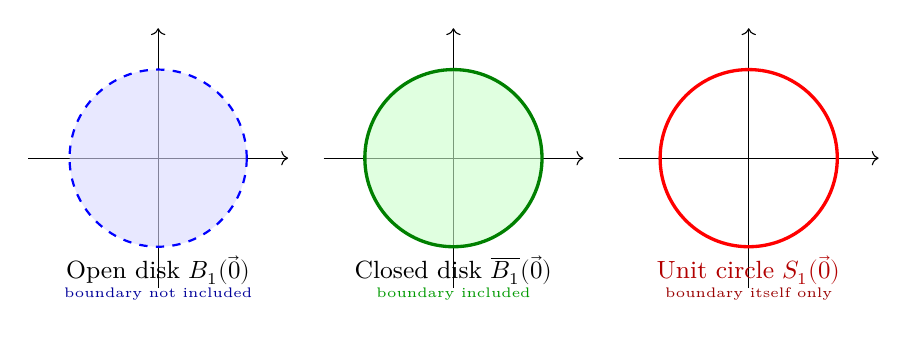
\begin{tikzpicture}[scale=0.75]

% --- Open Unit Disk ---
\begin{scope}[xshift=-5cm]
\draw[->] (-2.2,0)--(2.2,0);
\draw[->] (0,-2.2)--(0,2.2);
\fill[blue!15, opacity=0.6] (0,0) circle (1.5);
\draw[blue, thick, dashed] (0,0) circle (1.5); % dashed to show boundary not included
\node at (0,-1.9) {\small Open disk $B_1(\vec{0})$};
\node[blue!60!black] at (0,-2.3) {\tiny boundary not included};
\end{scope}

% --- Closed Unit Disk ---
\begin{scope}[xshift=0cm]
\draw[->] (-2.2,0)--(2.2,0);
\draw[->] (0,-2.2)--(0,2.2);
\fill[green!20, opacity=0.6] (0,0) circle (1.5);
\draw[green!50!black, very thick] (0,0) circle (1.5); % solid boundary
\node at (0,-1.9) {\small Closed disk $\overline{B_1}(\vec{0})$};
\node[green!60!black] at (0,-2.3) {\tiny boundary included};
\end{scope}

% --- Unit Circle ---
\begin{scope}[xshift=5cm]
\draw[->] (-2.2,0)--(2.2,0);
\draw[->] (0,-2.2)--(0,2.2);
\draw[red, very thick] (0,0) circle (1.5);
\node[red!70!black] at (0,-1.9) {\small Unit circle $S_1(\vec{0})$};
\node[red!60!black] at (0,-2.3) {\tiny boundary itself only};
\end{scope}

\end{tikzpicture}
\end{center}

\end{block}
\end{frame}

\begin{frame}{Unit Examples at the Origin}
\begin{block}{Case $n=3$:} (open unit ball, closed unit ball, unit sphere)
\begin{center}
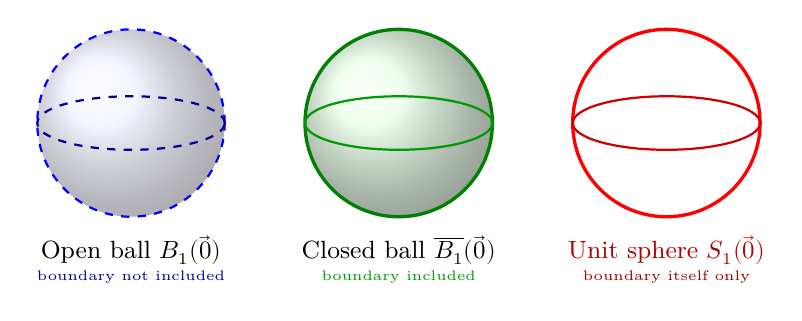
\begin{tikzpicture}[scale=0.85]
% --- Open Unit Ball ---
\begin{scope}[xshift=-4cm]
\shade[ball color=blue!10, opacity=0.5] (0,0) circle (1.4);
\draw[blue, dashed, thick] (0,0) circle (1.4); % dashed boundary = not included
\draw[blue!60!black, dashed, thick] (0,0) ellipse (1.4 and 0.4);
\node at (0,-1.9) {\small Open ball $B_1(\vec{0})$};
\node[blue!60!black] at (0,-2.3) {\tiny boundary not included};
\end{scope}
% --- Closed Unit Ball ---
\begin{scope}[xshift=0cm]
\shade[ball color=green!15, opacity=0.6] (0,0) circle (1.4);
\draw[green!50!black, very thick] (0,0) circle (1.4); % solid boundary
\draw[green!60!black, thick] (0,0) ellipse (1.4 and 0.4);
\node at (0,-1.9) {\small Closed ball $\overline{B_1}(\vec{0})$};
\node[green!60!black] at (0,-2.3) {\tiny boundary included};
\end{scope}
% --- Unit Sphere ---
\begin{scope}[xshift=4cm]
\shade[ball color=white, opacity=0] (0,0) circle (1.4);
\draw[red, very thick] (0,0) circle (1.4);
\draw[red!80!black, thick] (0,0) ellipse (1.4 and 0.4);
\node[red!70!black] at (0,-1.9) {\small Unit sphere $S_1(\vec{0})$};
\node[red!60!black] at (0,-2.3) {\tiny boundary itself only};
\end{scope}
\end{tikzpicture}
\end{center}
\end{block}
\end{frame}


\begin{frame}{Open/Closed $n$-Bricks}
\vspace{-0.3cm}
\begin{block}{Parallelotopes}
Let $n\in\mathbb{N}$ and $a_i<b_i$ for $i=1,\dots,n$.\\
Open $n$–brick: $(a_1,b_1)\times(a_2,b_2)\times\cdots\times(a_n,b_n),$\\
Closed $n$–brick: $[a_1,b_1]\times[a_2,b_2]\times\cdots\times[a_n,b_n],$\\
and Boundary:
\vspace{-0.3cm}
\begin{align*}
\partial\bigl([a_1,b_1]\times\cdots\times[a_n,b_n]\bigr)
=& \bigcup_{k=1}^n
\left([a_1,b_1]\times\cdots\times[a_{k-1},b_{k-1}]\times\{a_k,b_k\}
\right.\\
&\left.
\times[a_{k+1},b_{k+1}]\times\cdots\times[a_n,b_n]\right) \\
=& \Big(\{a_1,b_1\}\times[a_2,b_2]\times\cdots\times[a_n,b_n]\Big) \\
&\quad \cup \Big([a_1,b_1]\times\{a_2,b_2\}\times\cdots\times[a_n,b_n]\Big) \\
&\quad \cup \cdots \cup \Big([a_1,b_1]\times[a_2,b_2]\times\cdots\times\{a_n,b_n\}\Big).
\end{align*}
\end{block}
\end{frame}

%
\begin{frame}{Open and Closed 2D Bricks }
\vspace{-0.2cm}
\begin{block}{Case $n=2$: unit brick $(0,1)^2$ and $[0,1]^2$ (Squares/Rectangles)}
\begin{itemize}
\item Open square $(0,1)^2$: interior points only (boundary excluded).
\item Closed square $[0,1]^2$: includes all boundary edges.
\item Boundary $\partial[0,1]^2$: the four edges forming the perimeter.
\end{itemize}
\end{block}

\begin{center}
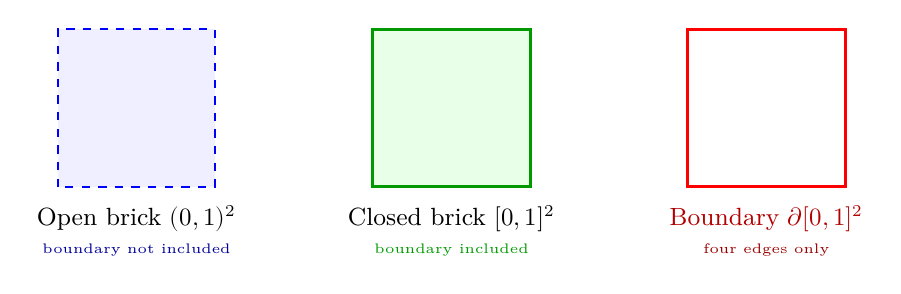
\begin{tikzpicture}[scale=1.0]
% --- Open square ---
\begin{scope}[xshift=-4cm]
\fill[blue!10, opacity=0.6] (0,0) rectangle (2,2);
\draw[blue, dashed, thick] (0,0) rectangle (2,2);
\node at (1,-0.4) {\small Open brick $(0,1)^2$};
\node[blue!60!black] at (1,-0.8) {\tiny boundary not included};
\end{scope}

% --- Closed square ---
\begin{scope}[xshift=0cm]
\fill[green!15, opacity=0.6] (0,0) rectangle (2,2);
\draw[green!60!black, very thick] (0,0) rectangle (2,2);
\node at (1,-0.4) {\small Closed brick $[0,1]^2$};
\node[green!60!black] at (1,-0.8) {\tiny boundary included};
\end{scope}

% --- Boundary only ---
\begin{scope}[xshift=4cm]
\draw[red, very thick] (0,0) rectangle (2,2);
\node[red!70!black] at (1,-0.4) {\small Boundary $\partial[0,1]^2$};
\node[red!60!black] at (1,-0.8) {\tiny four edges only};
\end{scope}
\end{tikzpicture}
\end{center}
\end{frame}

% (Cubes/Parallelepipeds)
\begin{frame}{Open and Closed 3D Bricks}
\vspace{-0.3cm}
\begin{block}{Case $n=3$: unit brick $(0,1)^3$ and $[0,1]^3$}
\begin{itemize}
\item Open cube $(0,1)^3$: interior points only (no faces).
\item Closed cube $[0,1]^3$: includes interior and all 6 faces.
\item Boundary $\partial[0,1]^3$: the 6 faces listed below:
\[
\{0,1\}\!\times\![0,1]\!\times\![0,1],\quad
[0,1]\!\times\!\{0,1\}\!\times\![0,1],\quad
[0,1]\!\times\![0,1]\!\times\!\{0,1\}.
\]
\end{itemize}
\end{block}
\vspace{-0.3cm}
\begin{center}
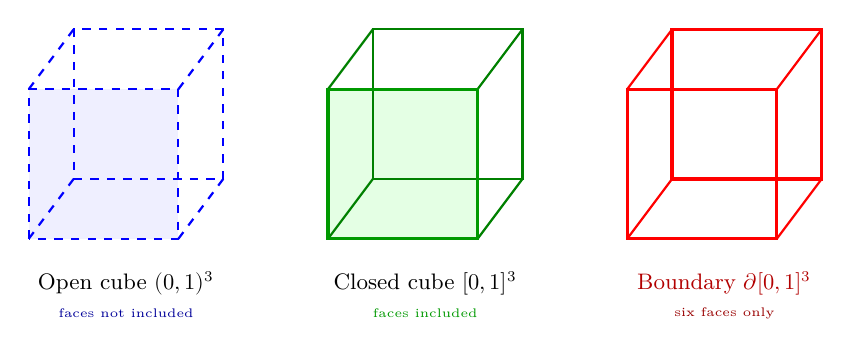
\begin{tikzpicture}[scale=0.95, every node/.style={scale=0.9}]
% --- Open cube ---
\begin{scope}[xshift=-4cm]
\fill[blue!10, opacity=0.6] (0,0) rectangle (2,2);
\draw[blue, dashed, thick] (0,0) rectangle (2,2);
\draw[blue, dashed, thick] (0,0) -- (0.6,0.8);
\draw[blue, dashed, thick] (2,0) -- (2.6,0.8);
\draw[blue, dashed, thick] (2,2) -- (2.6,2.8);
\draw[blue, dashed, thick] (0,2) -- (0.6,2.8);
\draw[blue, dashed, thick] (0.6,0.8) -- (2.6,0.8) -- (2.6,2.8) -- (0.6,2.8) -- cycle;
\node at (1.3,-0.6) {\small Open cube $(0,1)^3$};
\node[blue!60!black] at (1.3,-1.0) {\tiny faces not included};
\end{scope}

% --- Closed cube ---
\begin{scope}[xshift=0cm]
\fill[green!15, opacity=0.7] (0,0) rectangle (2,2);
\draw[green!50!black, thick] (0,0) -- (0.6,0.8);
\draw[green!50!black, thick] (2,0) -- (2.6,0.8);
\draw[green!50!black, thick] (2,2) -- (2.6,2.8);
\draw[green!50!black, thick] (0,2) -- (0.6,2.8);
\draw[green!50!black, thick] (0.6,0.8) -- (2.6,0.8) -- (2.6,2.8) -- (0.6,2.8) -- cycle;
\draw[green!60!black, very thick] (0,0) rectangle (2,2);
\node at (1.3,-0.6) {\small Closed cube $[0,1]^3$};
\node[green!60!black] at (1.3,-1.0) {\tiny faces included};
\end{scope}

% --- Boundary only ---
\begin{scope}[xshift=4cm]
\draw[red, thick] (0,0) -- (0.6,0.8);
\draw[red, thick] (2,0) -- (2.6,0.8);
\draw[red, thick] (2,2) -- (2.6,2.8);
\draw[red, thick] (0,2) -- (0.6,2.8);
\draw[red, very thick] (0,0) rectangle (2,2);
\draw[red, very thick] (0.6,0.8) -- (2.6,0.8) -- (2.6,2.8) -- (0.6,2.8) -- cycle;
\node[red!70!black] at (1.3,-0.6) {\small Boundary $\partial[0,1]^3$};
\node[red!60!black] at (1.3,-1.0) {\tiny six faces only};
\end{scope}
\end{tikzpicture}
\end{center}
\end{frame}



\begin{frame}{Interior and Boundary Points}
\begin{block}{Definition}
    Let $n \in \mathbb{N}$, and let $M \subseteq \mathbb{R}^n$.

    \textbf{1. Interior Point}

    A point $x \in M$ is interior to $M$ if there exists an open ball (equivalently, an open brick) $U$ such that $x \in U \subseteq M$.

    \vspace{0.5em}

    \textbf{2. Boundary Point}

    A point $x \in \mathbb{R}^n$ is a boundary point of $M$ if for every open neighborhood $U$ containing $x$, the following two conditions hold:
    $$U \cap M \neq \varnothing \quad \text{and} \quad U \cap (\mathbb{R}^n \setminus M) \neq \varnothing.$$
\end{block}
\end{frame}

\begin{frame}{Interior and Boundary Points}
\textbf{Examples in $\mathbb{R}^2$.}
\begin{align*}
M_1 = B_1(0,0) = \{(x,y)\mid x^2+y^2<1\}: \text{ every point is interior.}\\
M_2 = \overline{B_1}(0,0): \text{ interior points are those with }x^2+y^2<1,\\
\text{boundary points are those on the unit circle }x^2+y^2=1.
\end{align*}
\vspace{-0.3cm}
\begin{center}
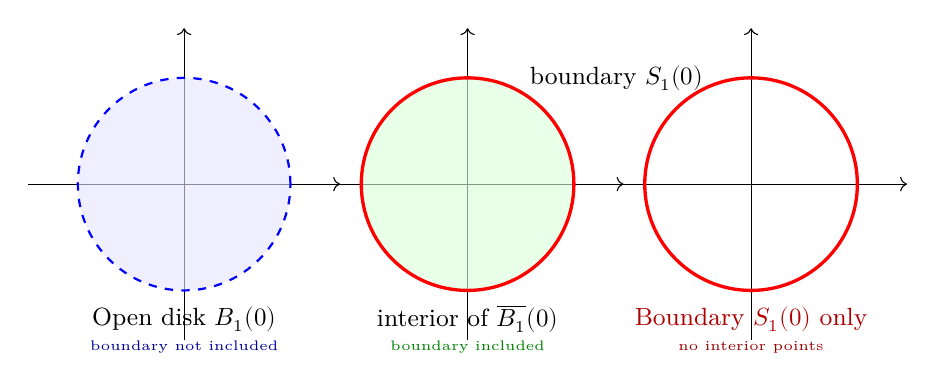
\begin{tikzpicture}[scale=0.9]

% --- Open Unit Disk ---
\begin{scope}[xshift=-4cm]
\draw[->] (-2.2,0)--(2.2,0);
\draw[->] (0,-2.2)--(0,2.2);
\fill[blue!10, opacity=0.6] (0,0) circle (1.5);
\draw[blue, dashed, thick] (0,0) circle (1.5);
\node at (0,-1.9) {\small Open disk $B_1(0)$};
\node[blue!60!black] at (0,-2.3) {\tiny boundary not included};
\end{scope}

% --- Closed Unit Disk (with boundary) ---
\begin{scope}[xshift=0cm]
\draw[->] (-2.2,0)--(2.2,0);
\draw[->] (0,-2.2)--(0,2.2);
\fill[green!15, opacity=0.6] (0,0) circle (1.5);
\draw[very thick, red] (0,0) circle (1.5);
\node at (2.1,1.5) {\small boundary $S_1(0)$};
\node at (0,-1.9) {\small interior of $\overline{B_1}(0)$};
\node[green!50!black] at (0,-2.3) {\tiny boundary included};
\end{scope}

% --- Boundary Only (Unit Circle) ---
\begin{scope}[xshift=4cm]
\draw[->] (-2.2,0)--(2.2,0);
\draw[->] (0,-2.2)--(0,2.2);
\draw[red, very thick] (0,0) circle (1.5);
\node[red!70!black] at (0,-1.9) {\small Boundary $S_1(0)$ only};
\node[red!60!black] at (0,-2.3) {\tiny no interior points};
\end{scope}

\end{tikzpicture}
\end{center}

\end{frame}



\begin{frame}{Open and Closed Sets in $\mathbb{R}^n$}
\textbf{Definitions.} Let $M\subseteq\mathbb{R}^n$.
\begin{align*}
M \text{ is \emph{open}} &\iff \text{every }x\in M\text{ is interior.}\\
M \text{ is \emph{closed}} &\iff \mathbb{R}^n\setminus M \text{ is open.}
\end{align*}

\textbf{Basic examples and reasons.}
\begin{itemize}
\item $B_r(x)$ is open: for each $y\in B_r(x)$ take a smaller ball $B_\varepsilon(y)\subset B_r(x)$.
\item $\overline{B_r}(x)$ is closed: its complement is open (distance to $x$ is continuous; $\{d>r\}$ is open).
\item Open $n$-bricks are open (product of open intervals); closed $n$-bricks are closed (finite intersection of closed half-spaces).
\item $\mathbb{R}^n$ and $\varnothing$ are both open and closed: complements are $\varnothing$ and $\mathbb{R}^n$, respectively, which are open.
\end{itemize}
\end{frame}

\begin{frame}{Interior and Closure of a Set}
\begin{block}{Definitions.} For $M\subseteq\mathbb{R}^n$:
\begin{align*}
\operatorname{int}(M) :=& \text{the set of interior points of }M\ \ (\text{largest open subset of }M),\\
\overline{M} :=& \text{the smallest closed set containing }M\\ &(\text{intersection of all closed supersets}).
\end{align*}
\end{block}

\begin{block}{Example.} $M=[0,1)\subseteq\mathbb{R}$.
\begin{align*}
\operatorname{int}(M)=(0,1),\qquad \overline{M}=[0,1].
\end{align*}
\end{block}
\end{frame}

\begin{frame}{Relative (Subspace) Topology}
\begin{block}{Definition.}Let $M$ be a subset of $\mathbb{R}^n$ and $U$ be a subset of $M$. We define the relative topology on $M$ by setting its open and closed sets as follows:
\begin{align*}
U \text{ is \emph{open in $M$} } &\iff \exists\ \text{an open set }X\subseteq\mathbb{R}^n\\ &\text{such that } U=M\cap X.\\
U \text{ is \emph{closed in $M$} } &\iff \exists\ \text{a closed set }X\subseteq\mathbb{R}^n\\ &\text{such that } U=M\cap X.
\end{align*}
\end{block}


\end{frame}

\begin{frame}{Relative (Subspace) Topology}
\vspace{-0.2cm}
\textbf{Example ($n=2$).} $M=S^1=\{(x,y)\mid x^2+y^2=1\}$.
\vspace{-0.3cm}
\begin{center}
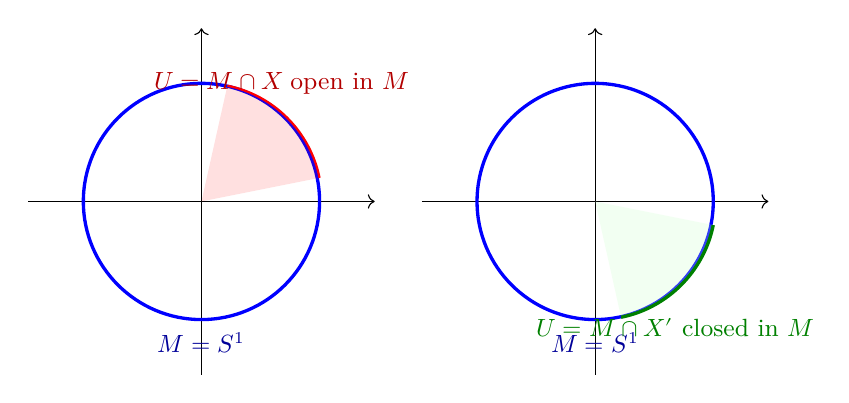
\begin{tikzpicture}[scale=1.0]

% --- Left: U = M ∩ X (open in M) ---
\begin{scope}[xshift=-2.5cm]
% Axes
\draw[->] (-2.2,0)--(2.2,0);
\draw[->] (0,-2.2)--(0,2.2);
% Circle S^1
\draw[very thick, blue] (0,0) circle (1.5);
% Open angular sector X (shaded)
\fill[red, opacity=0.12] (0,0)--(1.5,0.3) arc (11.5:78.5:1.5) -- (0,0)--cycle;
% Arc of intersection U = M ∩ X
\draw[red, thick] (1.5,0.3) arc (11.5:78.5:1.5);
\node[blue!60!black] at (0,-1.8) {\small $M=S^1$};
\node[red!70!black] at (1.0,1.5) {\small $U=M\cap X$ open in $M$};
\end{scope}

% --- Right: U = M ∩ X' (closed in M) ---
\begin{scope}[xshift=2.5cm]
% Axes
\draw[->] (-2.2,0)--(2.2,0);
\draw[->] (0,-2.2)--(0,2.2);
% Circle S^1
\draw[very thick, blue] (0,0) circle (1.5);
% Closed angular sector X' (shaded darker)
\fill[green!20, opacity=0.25] (0,0)--(1.5,-0.3) arc (-11.5:-78.5:1.5) -- (0,0)--cycle;
% Arc of intersection U = M ∩ X'
\draw[green!50!black, very thick] (1.5,-0.3) arc (-11.5:-78.5:1.5);
\node[blue!60!black] at (0,-1.8) {\small $M=S^1$};
\node[green!50!black] at (1.0,-1.6) {\small $U=M\cap X'$ closed in $M$};
\end{scope}
\end{tikzpicture}
\end{center}

\textit{Similarly:} If $X$ is closed (e.g.\ intersection with a closed half-plane), then $U=M\cap X$ is closed in $M$.

\textbf{Note.} Whether $M$ itself is open/closed in $\mathbb{R}^n$ is independent from being open/closed in $M$; any $M$ is both open and closed in the relative topology on $M$.
\end{frame}


\begin{frame}{Continuous vs.\ Smooth}
\vspace{-0.3cm}
\begin{block}{Smoothness on Open/Closed Domains}
\textbf{Continuous} means: small changes in input yield small changes in output (no derivatives required).
\textbf{Smooth} (infinitely differentiable) means: all partial derivatives of all orders exist and are continuous.
\end{block}

\vspace{-0.2cm}
\begin{block}{Definition (Smooth map on an open domain).}
Let $m,n\in\mathbb{N}$, $U\subseteq\mathbb{R}^m$ be open, $V\subseteq\mathbb{R}^n$, and $f=(f_1,\dots,f_n):U\to V$.
We say $f$ is \emph{smooth} (write $f\in C^\infty(U,V)$) if for every $k\in\mathbb{N}^+$, for all choices $i_1,\dots,i_k\in\{1,\dots,m\}$ and each $j\in\{1,\dots,n\}$, the mixed partial
\vspace{-0.2cm}
\begin{align*}
\frac{\partial^k f_j}{\partial x_{i_1}\cdots \partial x_{i_k}}(x)
\end{align*}
exists for every $x\in U$.
\end{block}
\end{frame}

\begin{frame}{Smoothness on a closed domain}
    \begin{block}{Definition}
If $U\subseteq\mathbb{R}^m$ is \emph{not open} (e.g.\ closed), we say $f:U\to V$ is smooth if there exist an open set $\widehat{U}\subseteq\mathbb{R}^m$ with $U\subseteq \widehat{U}$ and a smooth map $\widehat{f}\in C^\infty(\widehat{U},V)$ such that $\widehat{f}\!\restriction_{U}=f$.
\begin{center}
\begin{tikzpicture}[scale=1.0,>=latex]

% Nodes
\node (U) at (0,0) {$U$};
\node (Uhat) at (3.5,0) {$\widehat{U}$};
\node (V) at (3.5,-2.3) {$V$};

% Arrows
\draw[->] (U) -- (Uhat) node[midway, above] {\small incl};
\draw[->] (U) -- (V) node[midway, left=2pt] {\small $f$};
\draw[->] (Uhat) -- (V) node[midway, right=2pt] {\small $\widehat{f}\in C^{\infty}(\widehat{U},V)$};

% Optional alignment guide (invisible)
%\draw[dotted] (U) -- (3.5,0);

\end{tikzpicture}
\end{center}
\end{block}
\end{frame}

\begin{frame}{Examples}
\vspace{-0.3cm}
    \begin{itemize}
    \item \textbf{Elementary Functions:} The following are smooth ($C^\infty$ on their natural domains):
    \begin{itemize}
        \item \textbf{Polynomials} (on all of $\mathbb{R}$).
        \item \textbf{Trigonometric Functions:} $\sin(x)$ and $\cos(x)$ (on all of $\mathbb{R}$).
        \item \textbf{Exponential Function:} $\exp(x)$ (on all of $\mathbb{R}$).
        \item \textbf{Logarithm:} $\ln(x)$ (on its domain, $(0, \infty)$).
    \end{itemize}
    \begin{itemize}
        \item \textbf{Sums, Products, and Quotients} (where the denominator is non-zero).
        \item \textbf{Compositions:} If $f$ and $g$ are smooth, then $f \circ g$ is smooth.
    \end{itemize}
\end{itemize}

\begin{itemize}
    \item \textbf{A Function That Fails $C^1$ at a Point:}

    Consider the function $f(x) = |x|^{1/3}$.

    \item \textbf{The Issue:} This function is not $C^1$ at $x=0$.

    The derivative is $f'(x) = \frac{1}{3} |x|^{-2/3} \cdot \text{sgn}(x)$.
    \item \textbf{Conclusion:}
    $\lim_{x \to 0} |f'(x)| = \lim_{x \to 0} \frac{1}{3 |x|^{2/3}} = \infty.$ The derivative is not defined (it "blows up") at $x=0$, meaning $f(x)$ is not differentiable at this point, and thus cannot be $C^1$ there.
\end{itemize}
\end{frame}



\begin{frame}{Differential / Jacobian Matrix}
\textbf{Definition.} Let $m,n\in\mathbb{N}$, $U\subseteq\mathbb{R}^m$ open, $f=(f_1,\dots,f_n)\in C^\infty(U,\mathbb{R}^n)$ and $x=(x_1,\dots,x_m)\in U$.
The \emph{Jacobian (differential) at $x$} is the $n\times m$ matrix
\begin{align*}
D_x f
=\begin{pmatrix}
\frac{\partial f_1}{\partial x_1}(x) & \cdots & \frac{\partial f_1}{\partial x_m}(x)\\
\vdots & \ddots & \vdots\\
\frac{\partial f_n}{\partial x_1}(x) & \cdots & \frac{\partial f_n}{\partial x_m}(x)
\end{pmatrix}.
\end{align*}
It represents the best linear approximation to $f$ at $x$.

\textbf{Example (Polar coordinates).} $f:[0,1]\times[0,2\pi]\to \overline{B_1(0,0)}$, $f(r,\phi)=(r\cos\phi,\ r\sin\phi)$. Then
\begin{align*}
\frac{\partial f}{\partial r}(r,\phi)=(\cos\phi,\ \sin\phi),\qquad
\frac{\partial f}{\partial \phi}(r,\phi)=(-r\sin\phi,\ r\cos\phi).
\end{align*}
Hence
\begin{align*}
D_{(r,\phi)} f
=\begin{pmatrix}
\cos\phi & -\,r\sin\phi\\
\sin\phi & \ \ r\cos\phi
\end{pmatrix},\qquad
\det D_{(r,\phi)} f = r.
\end{align*}
\end{frame}

\begin{frame}{Inverse Function Theorem (IFT)}
\vspace{-0.3cm}
\begin{block}{Theorem}
Let $m\in\mathbb{N}$, $U\subseteq\mathbb{R}^m$ open, and $f\in C^\infty(U,\mathbb{R}^m)$.
If at $x_0\in U$ the Jacobian $D_{x_0}f$ is invertible (i.e.\ $\det D_{x_0}f\neq 0$), then there exist open neighborhoods $x_0\in U_0\subseteq U$ and $f(x_0)\in V_0\subseteq\mathbb{R}^m$ such that
\begin{align*}
f\!\restriction_{U_0}:U_0\to V_0
\end{align*}
is a \emph{diffeomorphism} (bijective, smooth inverse).

\end{block}

\textbf{Proof (complete outline with key steps).}
\begin{itemize}
\item \emph{Reduction:} By translation and linear change of variables (compose with $D_{x_0}f^{-1}$) assume $x_0=0$, $f(0)=0$, $D_0 f = I$.
\item \emph{Fixed-point map:} For $y$ near $0$, define $T_y(x)=x-(f(x)-y)$. Then $T_y(0)=y$ and $D T_y(0)=I-D f(0)=0$.
\end{itemize}
\end{frame}

\begin{frame}{Proof}
\begin{itemize}
\item \emph{Contraction:} Using continuity of $Df$ at $0$, choose a small ball where $\|Df(x)-I\|\le \frac12$, so $T_y$ is a contraction on that ball for all $y$ in a small ball. By Banach’s fixed-point theorem, $T_y$ has a unique fixed point $x$, i.e.\ $f(x)=y$.
\item \emph{Regularity:} The fixed point depends smoothly on $y$ (by implicit function theorem/contractive mapping with parameters), giving $f^{-1}\in C^\infty(V_0,U_0)$.
\end{itemize}
\end{frame}

\begin{frame}{Example}
\begin{block}{Polar-annulus example.} Let $U=(\frac{1}{2},1)\times(0,2\pi)$ and define
\begin{align*}
f(r,\phi)=(r\cos\phi,\ r\sin\phi).
\end{align*}
Then $D f$ is as before, $\det D f=r\in(\frac{1}{2},1)$, so $f$ is a local diffeomorphism everywhere on $U$.
Its image is the open annulus
\begin{align*}
V=\{(x,y)\in\mathbb{R}^2\mid \tfrac14<x^2+y^2<1\}\setminus\{(x,0):x>0\},
\end{align*}
where the ray $\{(x,0):x>0\}$ is removed to keep the angular coordinate single-valued. On $U$ we have a global diffeomorphism $f:U\overset{\sim}{\longrightarrow} V$.

\end{block}
\end{frame}


\begin{frame}{Immersions: Curves and Surfaces}
\begin{block}{Definition (Immersion).}
Let $m,n\in\mathbb{N}$, $U\subseteq\mathbb{R}^m$ open, $V\subseteq\mathbb{R}^n$, and $f\in C^\infty(U,V)$.
We say $f$ is an \emph{immersion} if for all $x\in U$, the Jacobian $D_x f\in M_{n\times m}(\mathbb{R})$ has \emph{rank $m$} (its $m$ columns are linearly independent).
\end{block}

\begin{block}{Specific case.}
\begin{itemize}
\item $m=1$ (parametrized curve): $f(t)=(f_1(t),\dots,f_n(t))$. Then
\begin{align*}
D_t f = \begin{pmatrix} f_1'(t)\\ \vdots\\ f_n'(t)\end{pmatrix},
\qquad
f \text{ immersion } \Leftrightarrow D_t f \neq 0 \ \text{ for all } t.
\end{align*}
\end{itemize}
\end{block}
\end{frame}

\begin{frame}{Example}
\begin{itemize}
\item $m=2$, $n=3$ (parametrized surface):
$f(x_1,x_2)=(f_1(x_1,x_2),f_2(x_1,x_2),f_3(x_1,x_2))$ with
\begin{align*}
D_{(x_1,x_2)} f
=\begin{pmatrix}
\frac{\partial f_1}{\partial x_1} & \frac{\partial f_1}{\partial x_2} \\[4pt]
\frac{\partial f_2}{\partial x_1} & \frac{\partial f_2}{\partial x_2} \\[4pt]
\frac{\partial f_3}{\partial x_1} & \frac{\partial f_3}{\partial x_2}
\end{pmatrix}
=\big(\,\frac{\partial f}{\partial x_1}\ \ \frac{\partial f}{\partial x_2}\,\big),
\end{align*}
so $\operatorname{rank} D f=2 \Leftrightarrow \frac{\partial f}{\partial x_1}$
and $\frac{\partial f}{\partial x_2}$ are linearly independent in $\mathbb{R}^3$.
Equivalently, all $2\times 2$ minors
\begin{align*}
b_1=\det\!
\begin{pmatrix}
\frac{\partial f_2}{\partial x_1} & \frac{\partial f_2}{\partial x_2} \\[4pt] 
\frac{\partial f_3}{\partial x_1} & \frac{\partial f_3}{\partial x_2}
\end{pmatrix},
b_2=\det\!
\begin{pmatrix}
\frac{\partial f_3}{\partial x_1} & \frac{\partial f_3}{\partial x_2} \\[4pt] 
\frac{\partial f_1}{\partial x_1} & \frac{\partial f_1}{\partial x_2}
\end{pmatrix},
b_3=\det\!
\begin{pmatrix}
\frac{\partial f_1}{\partial x_1} & \frac{\partial f_1}{\partial x_2} \\[4pt]
\frac{\partial f_2}{\partial x_1} & \frac{\partial f_2}{\partial x_2}
\end{pmatrix}
\end{align*}
do not vanish simultaneously (equivalently
$\frac{\partial f}{\partial x_1} \times \frac{\partial f}{\partial x_2} \neq 0$).
\end{itemize}
\end{frame}

\begin{frame}{Spherical Coordinates}
\vspace{-0.2cm}
\begin{block}{Immersion of $S^2$}
\textbf{Parametrization.} Let $(\theta,\varphi)\in(0,\pi)\times(0,2\pi)$ and define
\vspace{-0.3cm}
\begin{align*}
f(\theta,\varphi)
=\big(\sin\theta\cos\varphi,\ \sin\theta\sin\varphi,\ \cos\theta\big).
\end{align*}
Then
\vspace{-0.3cm}
\begin{align*}
\partial f / (\partial \theta)&=(\cos\theta\cos\varphi,\ \cos\theta\sin\varphi,\ -\sin\theta)^T,\\
\partial f / (\partial \varphi)&=(-\sin\theta\sin\varphi,\ \sin\theta\cos\varphi,\ 0)^T.
\end{align*}
\textbf{Rank condition.} The $3\times 2$ Jacobian $[\ \partial f / (\partial \theta)\ \ \partial f / (\partial \varphi)\ ]$ has rank $2$ whenever $\sin\theta\neq 0$, i.e.\ for $\theta\in(0,\pi)$, hence $f$ is an immersion on that open strip.\\
\textbf{Singularities (poles).} At $\theta=0$ (north pole) or $\theta=\pi$ (south pole), $\sin\theta=0$ and thus $\partial f / (\partial \varphi)=0$, so $\operatorname{rank} Df \le 1$; these are \emph{singular points} for this chart.
\end{block}
\end{frame}



\begin{frame}{Spherical Coordinates}
\begin{block}{Geometry.}
\begin{itemize}
\item Fixing $\varphi$ traces a \emph{meridian} (e.g.\ the Greenwich meridian at $\varphi=0$).
\item Fixing $\theta$ traces a \emph{parallel} (latitude circle); $\theta=\pi/2$ is the equator.
\end{itemize}

\textbf{Charts.} The sphere needs at least two charts to avoid the pole singularities; e.g.\ one chart missing the north pole and one missing the south pole.
\end{block}
\end{frame}

\begin{frame}{Summary}

\vspace{-0.2cm}
\begin{block}{}
    \begin{itemize}
\item Defined open and closed balls, spheres, and $n$–bricks (open, closed, boundary).
  \item Distinguished between interior, boundary, and exterior points of subsets $M\subseteq\mathbb{R}^n$.
  \item Defined open and closed sets, interiors, closures, and complements.
  \item Introduced relative (subspace) topology: sets open or closed in $M$ via intersections with open/closed subsets of $\mathbb{R}^n$.
  \item Illustrated with visual examples in $\mathbb{R}^1$, $\mathbb{R}^2$, and $\mathbb{R}^3$ (segments, disks, cubes, spheres).
\end{itemize}
\end{block}
\end{frame}

\begin{frame}{Summary}

\vspace{-0.2cm}
\begin{block}{}
    \begin{itemize}
\item Smooth maps on open sets have derivatives of all orders; on non-open sets they are defined by smooth extension to an open neighborhood.
\item The Jacobian $D_x f$ captures the best linear approximation; in polar coordinates $\det D f=r$.
\item Inverse Function Theorem: if $\det D_{x_0}f\neq 0$, then $f$ is locally a diffeomorphism; polar map on an annulus is a model example.
\item Immersion $U\to\mathbb{R}^n$: full column rank Jacobian; curves require nonzero velocity; surfaces require $f_u,f_v$ independent ($f_u\times f_v\neq 0$).
\item Spherical chart is immersive off the poles; poles are chart singularities necessitating multiple charts to cover $S^2$.
\end{itemize}
\end{block}
\end{frame}

\begin{frame}{Thanks}
  \cmcendframe
\end{frame}

\end{document}
